% !TEX root = ../main.tex

\chapter{基于偏好联盟博弈的分布式任务分配方法}
\label{chap:hedonic}

\section{引言}
\label{hg:sec:intro}

使用偏好联盟博弈模型(Hedonic Coalition Game, HCG)解决任务分配问题的思路是将任务分配问题看作是智能体划分问题,按照任务或目标的不同划分联盟,每个智能体对不同联盟有着不同的偏好,智能体会根据自己的偏好选择自己的联盟,最终所有智能体在确定了自己的所属联盟后,便得到了任务分配的解。本章将建立基于HCG的任务分配框架并提出对应求解算法,并通过仿真对比实验验证其有效性。


% ---------------------
% ---------------------
\section{偏好联盟博弈模型}
\label{hcg:sec:hcgmodel}

在介绍HCG模型概念之前,需要先在第\ref{chap:model}章建立的模型的基础上进行一些修正。沿用第\ref{chap:model}章中的符号和定义,智能体集合为$\mathcal{M}=\{\mathcal{M}_1,\dots,\mathcal{M}_{n_m}\}$,任务集合为$\mathcal{T} = \{\mathcal{T}_0,\mathcal{T}_1,\dots,\mathcal{T}_{n_t}\}$。在此章中,不再使用任务效用函数概念,而每个智能体拥有一个智能体效用函数,因此可将智能体效用函数简记为$U_i(\mathcal{T}_j,p):\mathcal{T} \times |\mathcal{M}| \mapsto \mathbb{R}$,这里的智能体效用函数与第\ref{chap:pg}章中使用WLU定义的智能体效用函数不同,除了与当前分配的任务$\mathcal{T}_j$有关外,还与同时选择该任务的智能体个数$p$有关。对于$\mathcal{T}_0$,定义$U_i(\mathcal{T}_0,n)=0,\forall \mathcal{M}_i \in \mathcal{M}, 0 \leq n \leq n_m$。设当前分配解为$a=(a_1,a_2,\dots,a_{n_m})$,全局效用函数被定义为

\begin{equation}
\label{hcg:eq:gloablU}
	U_g(a) = \sum_{\mathcal{M}_i \in \mathcal{M}} U_i(a_i,p_j),
\end{equation}
其中
\begin{equation}
\label{hcg:eq:parcitipants}
	p_j = \sum_{\mathcal{M}_i \in \mathcal{M}} I\{a_i = \mathcal{T}_j\},\ \mathcal{T}_j \in \mathcal{T}.
\end{equation}

为了建立HCG模型,现引入如下概念。

\begin{definition}[偏好关系]
	对于每个智能体$\mathcal{M}_i$,将二元组$x=(\mathcal{T}_j,p)$称为一组联盟对,意味着“智能体$\mathcal{M}_i$将与$p$个队友一起执行任务$\mathcal{T}_j$”,记所有联盟对集合为$\mathcal{X}=\mathcal{T}\times\{1,\dots,n_m\}$。在所有联盟对上定义一个关于效用的偏序关系$\succ_i$,对任意$x_1,x_2 \in \mathcal{X}$,$x_1 \succ_i x_2$意味着智能体$\mathcal{M}_i$对联盟对$x_1$有较强的偏好,此外还可定义$x_1 \sim_i x_2$为智能体$\mathcal{M}_i$对$x_1$和$x_2$的偏好无差别,$x_1 \succeq_i x_2$意味着智能体$\mathcal{M}_i$对联盟对$x_1$有较弱的偏好。
\end{definition}

结合之前定义的智能体效用函数,偏好关系$\succ_i$可以定义为
\begin{equation}
\label{hcg:eq:preference}
	(\mathcal{T}_1,p_1) \succ_i (\mathcal{T}_2,p_2),\quad \text{if}\ U_i(\mathcal{T}_1,p_1) > U_i(\mathcal{T}_2,p_2).
\end{equation}

HCG模型$\mathcal{G}=(\mathcal{M},\mathcal{T},\succeq_i)$是由智能体集合,任务集合和智能体的偏好关系组成的博弈模型。在HCG模型框架下解决任务分配问题,实质上是将任务分配问题看做是对智能体的分组问题,智能体可根据自己的偏好自行选择加入某个联盟小组,下面的定义引入了任务分配中智能体联盟的概念。


\begin{definition}[联盟划分]
	对于HCG模型$\mathcal{G}$,定义一个集合$\Pi = \{S_0,S_1,\dots,S_{n_t}\}$,其中元素联盟集合$S_j \subseteq \mathcal{M},j=1,\dots,n_m$为同时选择任务$\mathcal{T}_j$的所有智能体集合,特别地,$S_0$代表该智能体没有选择任何任务。由于每个智能体智能选择一个任务,因此$\cup_{j=0}^{n_t} S_j = \mathcal{M},\ S_i \cap S_j =\emptyset,\ i \neq j$。为了后续论述方便,用$\Pi(i)$表示智能体$\mathcal{M}_i$选择的任务序号,用$S_{\Pi(i)}$表示智能体$\mathcal{M}_i$所属的联盟集合,即$S_{\Pi(i)}=\{S_j \in \Pi|\mathcal{M}_i \in S_j\}$。
\end{definition}

\begin{figure}[!htp]
  \centering
  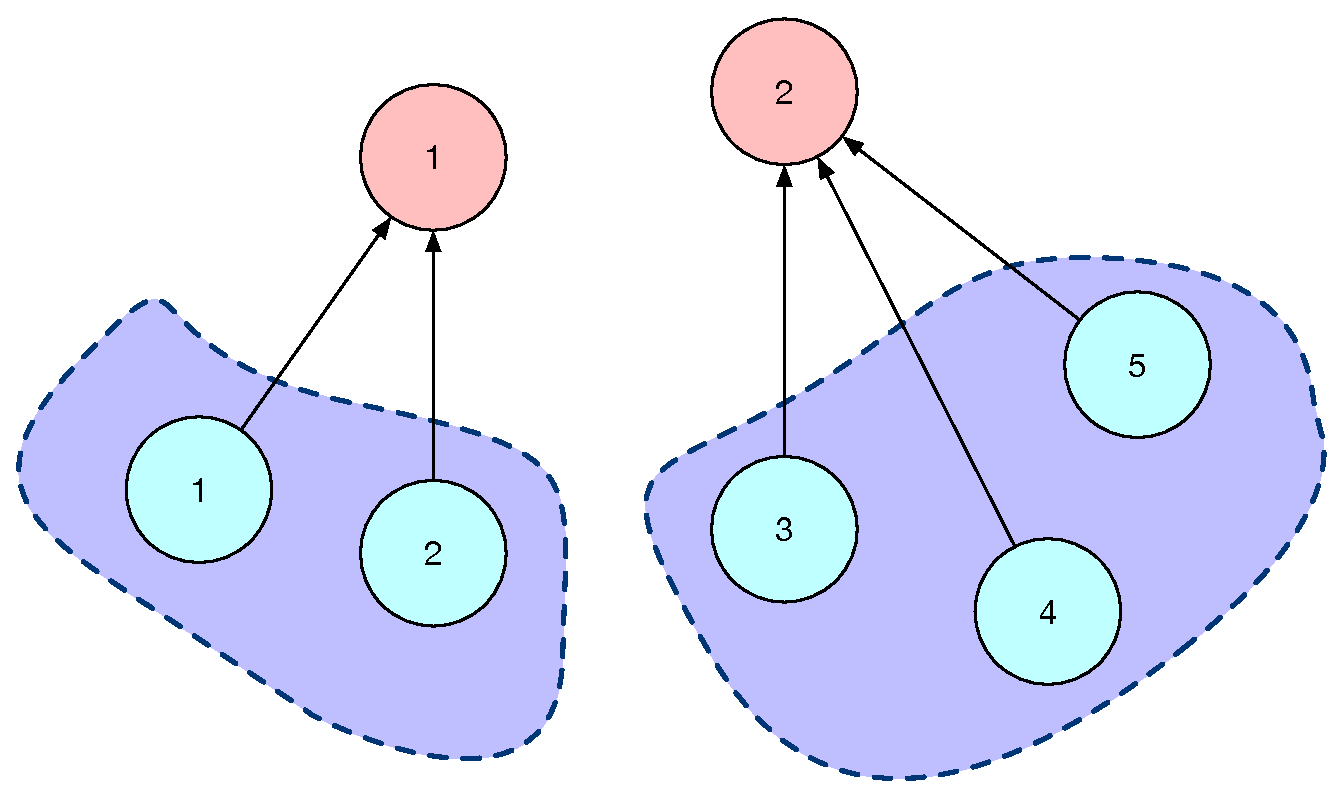
\includegraphics[height=5cm]{联盟划分.eps}
  \bicaption[联盟划分]
    {联盟划分}
    {Partition of coalition}
  \label{fig:partition}
\end{figure}

如图\ref{fig:partition}所示,智能体1,2(蓝色)同时选择目标1(红色),因此组成了一个联盟,同理智能体3,4,5组成了关于目标2的联盟。当所有智能体确定自己的联盟后,即可得到一组任务分配方案。有了联盟划分的概念,便可引入HCG模型下的纳什均衡概念。

\begin{definition}[HCG模型的纳什均衡]
	当在划分$\Pi$下,对于任意智能体$\mathcal{M}_i \in \mathcal{A}$都有
	\begin{equation}
	\label{hcg:eq:nash_stable}
		(t_{\Pi(i)},|S_{\Pi(i)}|) \succeq_i (t_j,|S_j \cup \{a_i\}|),\quad \forall S_j \in \Pi,
	\end{equation}
	则划分$\Pi$被称为是纳什均衡划分.
\end{definition}

定义中$S_j\cup \{a_i\}$是指智能体离开当前联盟加入新的联盟。因此,在联盟的概念下,HCG模型的纳什均衡状态意味着每个智能体均根据自身的效用函数选择自己最“喜爱”的联盟,在此状态下,所有智能体不会产生离开当前联盟的动力,此时也就得到了任务分配的稳定方案。



% ------------------------------------
% ------------------------------------
\section{面向任务分配的偏好联盟博弈模型设计}
\label{hcg:HGTA}


针对任务分配问题建立的HCG模型需要解决智能体效用函数设计问题。若采用式(\ref{hcg:eq:preference}) 定义的偏好关系,则智能体效用函数直接关系着智能体的偏好关系。因此首先为了保证HCG模型纳什均衡状态存在的必然性,需要对智能体效用函数$U_i(\mathcal{T}_j,p)$做出一定的要求。

\begin{definition}[社交疏远性质]
\label{hcg:eq:spao}
	如果智能体的偏好关系满足对任意任务$\mathcal{T}_j \in \mathcal{T} \setminus \{\mathcal{T}_0\}$,
	\begin{equation}
	\label{hcg:eq:spaoPrefer}
		(\mathcal{T}_j,p_1) \succeq_i (\mathcal{T}_j,p_2),\quad p_1 < p_2,\ p_1,p_2 \in \{1,\dots,n_m\},
	\end{equation}
	即智能体效用随着同联盟的成员数量增加而递减,则称该智能体具有社交疏远性质(Social Inhibition Characteristic, SIC)。若使用式(\ref{hcg:eq:preference})的定义,则SIC表现在智能体效用函数上为
	\begin{equation}
	\label{hcg:eq:spaoU}
		U_i(\mathcal{T}_j,p_1) > U_i(\mathcal{T}_j,p_2),\quad p_1<p_2,\ p_1,p_2 \in \{1,\dots,n_m\}.
	\end{equation}
\end{definition}

带有SIC的智能体组成的HCG模型一定存在纳什均衡。事实上有如下定理。

\begin{theorem}
	设HCG模型$\mathcal{G}=(\mathcal{M},\mathcal{T},\succeq_i)$中的智能体都具有SIC,则该模型一定存在纳什均衡。
	\begin{proof}
		可使用数学归纳法证明。当智能体数量$n_m=1$时,定理显然成立。
		
		假设$n_m=k$时,定理成立,即模型$\mathcal{G}=(\mathcal{M},\mathcal{T},\succeq_i)$存在纳什均衡。则当$n_m=k+1$时,新模型为$\widetilde{\mathcal{G}}=(\widetilde{\mathcal{M}},\mathcal{T},\succeq_i)$。设$\mathcal{M}_r \in \widetilde{\mathcal{M}}, \mathcal{M}_r \notin \mathcal{M}$,则$\widetilde{\mathcal{M}}=\mathcal{M} \cup \{\mathcal{M}_r\}$。
		
		对一个联盟划分$\Pi$,和任意的智能体$\mathcal{M}_i$,定义联盟可容纳额外成员数$\Delta_{\Pi(i)}$为当前联盟在不会使智能体$\mathcal{M}_i$不选择其他联盟的情况下,可额外增加的最大智能体个数,即
		\begin{equation}
		\label{hcg:eq:maxDelta}
			\Delta_{\Pi(i)}:= \min_{S_j \in \Pi \setminus \{S_{\Pi(i)}\}} \max_{\Delta \in \mathbb{Z}}\{\Delta|(\mathcal{T}_{\Pi(i)},|S_{\Pi(i)}|+\Delta) \succeq_i (\mathcal{T}_j, |S_j \cup \{\mathcal{M}_i\}|) \}.
		\end{equation}
		
		由SIC定义可知,$\Delta_{\Pi(i)}$满足以下性质:(1)如果划分$\Pi$是纳什均衡的,则对于任意智能体$\mathcal{M}_i$,有$\Delta_{\Pi(i)}\geq 0$;(2)如果$\Delta_{\Pi(i)}<0$,则智能体$\mathcal{M}_i$会选择离开当前联盟;(3)智能体$\mathcal{M}_i$在更换联盟后,设新联盟划分为$\Pi'$,则有$\Delta_{\Pi'(i)} \geq 0$。
		
		设$\Pi_0$是博弈$\mathcal{G}$的一个纳什均衡。当智能体$\mathcal{M}_r$选择了一个任务之后,会形成一个新的联盟划分$\Pi_1$,由第(3)点性质可知,$\Delta_{\Pi_1(r)}\geq 0$。此时若不存在智能体$\mathcal{M}_q \in \mathcal{A}$,使得$\Delta_{\Pi_1(q)}<0$,则可知划分$\Pi_1$是一个纳什均衡。
		
		假设此时至少存在一个智能体$\mathcal{M}_q$满足$\Delta_{\Pi_1(q)}<0$,则该智能体必定在$\mathcal{M}_r$所在的联盟中。由于此时智能体$\mathcal{M}_q$会选择另一个联盟加入,并再次形成一个新的联盟划分$\Pi_2$,因此此时智能体$\mathcal{M}_r$满足$\Delta_{\Pi_2(r)} \geq 1$(因为在$\mathcal{M}_q$移动之前已经满足不小于0)。换句话说,此时$\mathcal{M}_r$将不会再改变自己的联盟,即使其他智能体不断的变换自己的联盟。这意味着至多经过$|\widetilde{\mathcal{M}}|$次迭代,在最终的划分$\widetilde{\Pi}$下,所有的智能体都会满足$\Delta_{\widetilde{\Pi}(i)}\geq 0$,因此$\widetilde{\Pi}$是一个纳什均衡。
		
		由于定理在$n_m=k+1$时成立,因此归纳可得原定理成立。
	\end{proof}
\end{theorem}

根据以上定理,结合第\ref{chap:model}章中的效用函数定义,定义本章使用的智能体效用函数为

\begin{equation}
\label{hcg:eq:agentU}
	U_i(\mathcal{T}_j,p) = \frac{r(\mathcal{T}_j,|S_j|)}{|S_j|} - c_i(\mathcal{T}_j)
\end{equation}

其中$r(\mathcal{T}_j,|S_j|)$为导弹和联盟成员一起攻击目标$\mathcal{T}_j$可获得的回报,并假设联盟所有成员平分任务回报。在空战场景中,攻击同一个目标的导弹数量越多,击中的目标的概率越大,但当数量超过一定界限时,再增加导弹数量对于目标的攻击起到的作用很小,即随着联盟成员的数量增加,导弹所得到的边际回报在递减。因此可定义任务回报函数$r(\mathcal{T}_j,|S_j|)$为

\begin{equation}
\label{hcg:eq:task_reward}
	r(\mathcal{T}_j,|S_j|) = r_j^0 \cdot \log_{\varepsilon_j} (|S_j|+\varepsilon_j-1),
\end{equation}
其中$r_j^0$代表联盟中只有一位成员时的回报值,本文采用的是式(\ref{model:eq:taskU})定义的任务效用函数,$\varepsilon_j>0$是一个正数,与边际回报的递减速率有关。该函数的图像如图\ref{hcg:fig:rewardfunc}(a)所示,图中$r_j^{\text{min}}=10, \varepsilon_j = 3$。将任务回报函数代入式(\ref{hcg:eq:agentU})可得智能体效用函数为

\begin{equation}
\label{hcg:eq:agentU_reward}
	U_i(\mathcal{T}_j,|S_j|) = \frac{r_j^0 \cdot \log_{\varepsilon_j} (|S_j|+\varepsilon_j-1)}{|S_j|} - c_i(\mathcal{T}_j),
\end{equation}

图\ref{hcg:fig:rewardfunc}(b)所示的是$r_j^{\text{min}}=10,\varepsilon_j=3$时的智能体效用函数图像,由图像可知,该智能体效用符合SIC要求。

\begin{figure}[!hbtp]
  \centering
  \bisubcaptionbox{任务回报函数}%
                  {Task reward function}%
                  {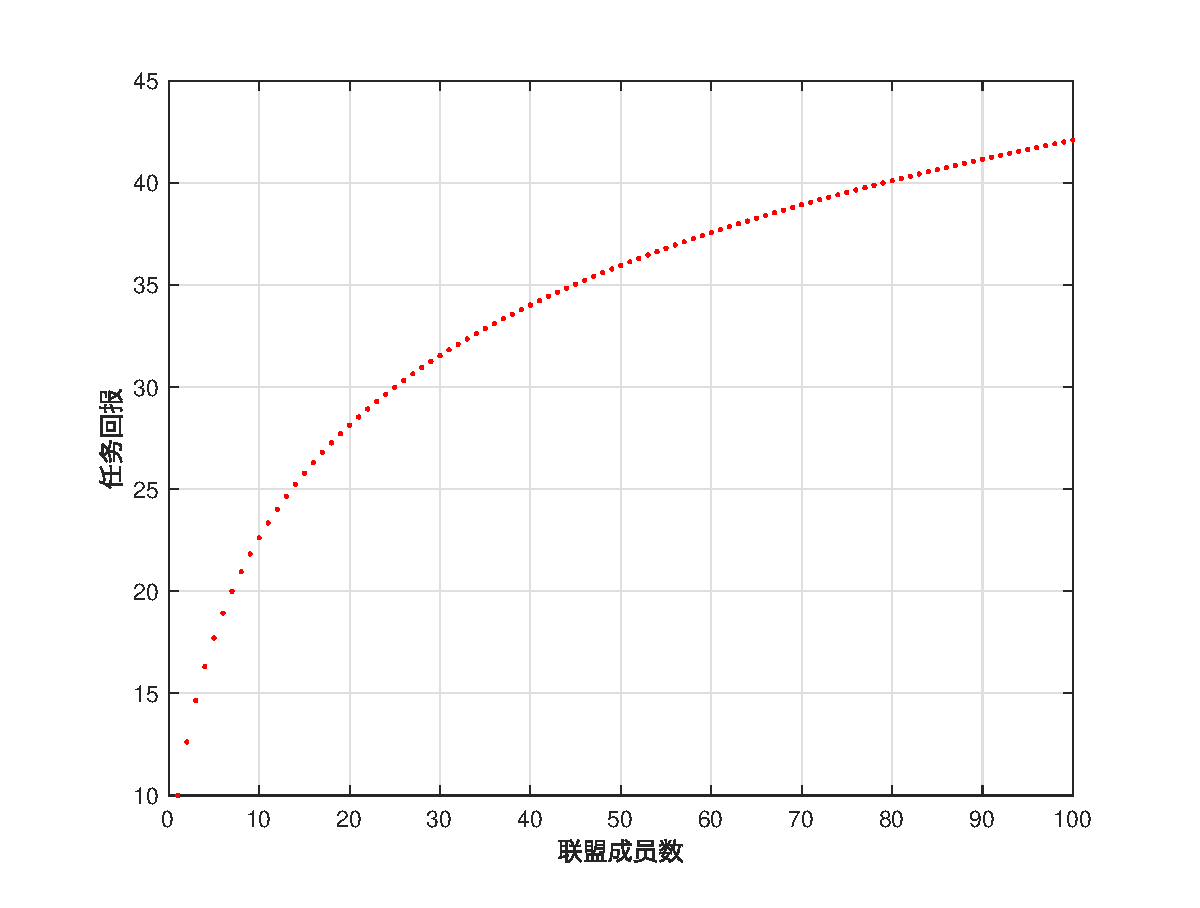
\includegraphics[height=5cm]{taskreward.eps}}
  \bisubcaptionbox{智能体回报函数}%
                  {Agent reward function}%
                  {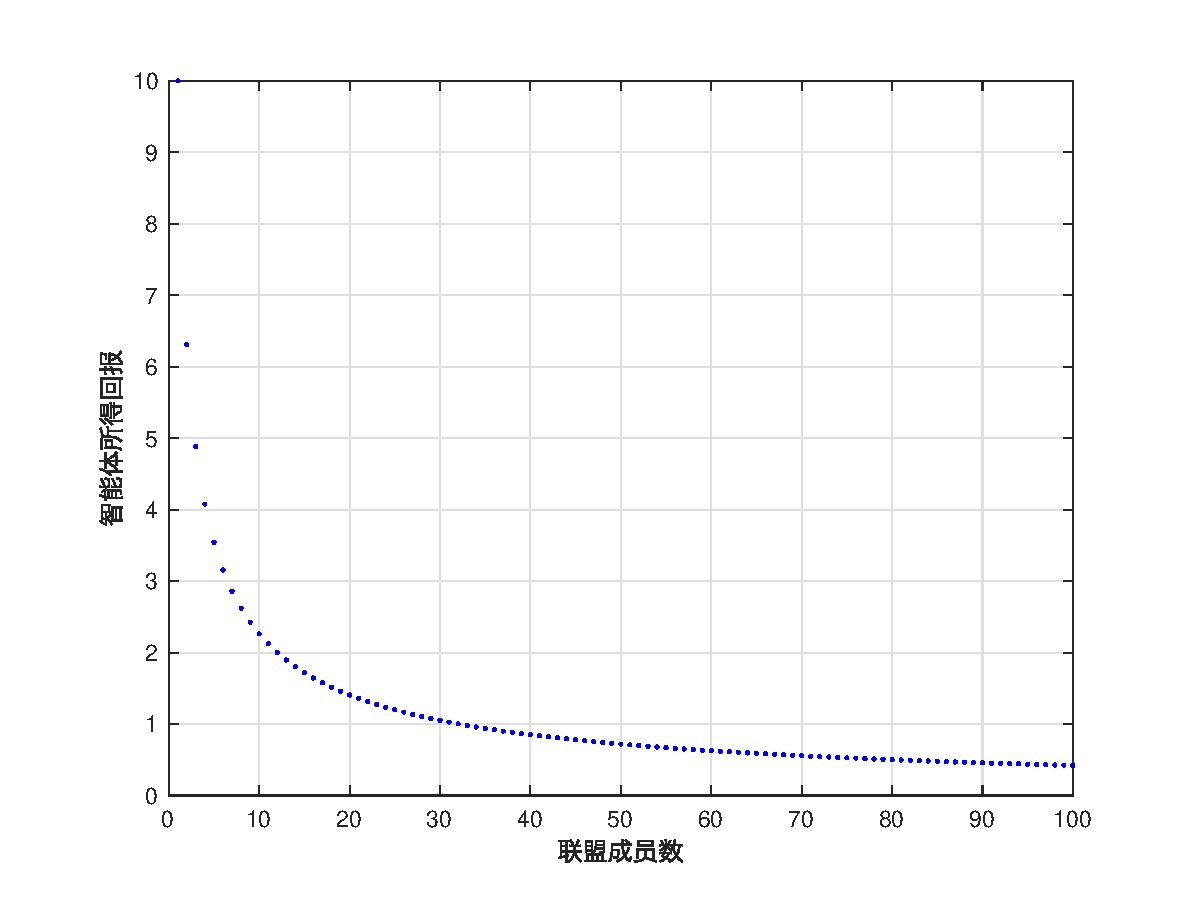
\includegraphics[height=5cm]{agentreward.eps}}
  \bicaption{HCG模型的回报函数}
            {Reward function of HCG model}
  \label{hcg:fig:rewardfunc}
\end{figure}

与第\ref{chap:pg}章中遇到的约束条件处理问题类似,在本章使用HCG模型的场景中,需要限定得到的联盟划分满足约束条件式(\ref{model:eq:bmax})。由于本节定义的智能体效用函数与联盟成员数有关,而约束条件也是对于执行同一任务的智能体个数的限定,因此可以直接对智能体效用函数进行进一步改进,使得智能体在加入一个联盟时,会考虑到加入该联盟后该联盟成员数是否仍满足约束条件。如果加入该联盟后约束条件不再满足,则智能体不会选择加入该联盟。具体来说,引入改进智能体效用函数$\widetilde U_i(\mathcal{T}_j,|S_j|)$为

\begin{equation}
\label{hcg:eq:modifiedAgentU}
	\widetilde U_i(\mathcal{T}_j,|S_j|) = 
	\begin{cases}
		U_i(\mathcal{T}_j,|S_j|),\ & \text{if $|S_j|\leq b_{\text{max}}^{(j)}$,}\\
		0,\ & \text{otherwise}
	\end{cases}
\end{equation}

当智能体即将选择加入的联盟已经达到约束边界时,若智能体加入,则得到的效用将会是0,因此智能体最终不会选择再加入该联盟,从而保证了求解的可行性。

%---------------------------
%---------------------------
\section{基于偏好联盟博弈模型的决策算法}
\label{hcg:decision}

\subsection{SAP算法}
在HCG模型下的智能体决策算法仍可使用第\ref{chap:pg}章\ref{pg:pgta:protocal}节中使用的几种决策算法,本节选择使用SAP算法,下面算法\ref{hcg:algo:HCGSAP}将直接给出使用SAP的HCG决策算法流程。算法中的$\text{CoWorkerNums}_j(k)$表示$k$时刻智能体$j$的联盟成员数量。为了适应HCG模型的需要,若智能体更换了联盟,则需要将自己更改联盟后新联盟和原有联盟更新后的成员数告诉其他智能体。

\begin{algorithm}[htb]
	\caption{使用SAP的HCG决策算法流程}
	\label{hcg:algo:HCGSAP}
	\small
	\SetAlgoLined
	\KwIn{$\mathcal{M},\mathcal{T},\mathcal{A},r$}
	\KwOut{均衡解$a^*$}
	\tcp{初始化参数}
	$k \gets 1$\;
	随机生成任务分配初始解$a(0)$\;
	\tcp{计算初始每个任务联盟的成员数}
	$\text{CoWorkerNums}_j(0) \gets \sum_{\mathcal{M}_i \in \mathcal{M}} I\{a_i(0)=\mathcal{T}_j\}$\;
	\While{true}{
		随机选择一个智能体$\mathcal{M}_i$\;
		$n_i=|\mathcal{A}_i|$\;
		\For{$j=1:n_t$}{
			根据式(\ref{hcg:eq:agentU_reward})计算$U_i(\mathcal{T}_j,|S_j|+1)$\;
		}
		根据式(\ref{pg:eq:sappdf})计算$p_i(k)$\;
		根据$p_i(k)$随机选择任务$\mathcal{T}_l$\;
		\tcp{更新联盟划分和联盟成员数}
		$a_i(k) \gets  \mathcal{T}_l$\;
		$\text{CoWorkerNums}_{a_i(k-1)}(k) \gets \text{CoWorkerNums}_{a_i(k-1)}(k) - 1$\;
		$\text{CoWorkerNums}_{a_i(k)}(k) \gets \text{CoWorkerNums}_{a_i(k)}(k) + 1$\;
		$k\gets k+1$\;
	}
\end{algorithm}

%----------------------------
\subsection{分布式一致性算法}

本节将提出HCG模型下的另一种决策算法,称为分布式一致性算法(Distribute Mutual Consistence Algorithm, DMCA)。MEA在每次迭代中,所有智能体都会做出自己的决策,但智能体在交互中会只保留一个智能体的决策结果。算法\ref{hcg:algo:decsion}和算法\ref{hcg:algo:DMCA}给出了使用DMCA决策算法的两个阶段,其中算法\ref{hcg:algo:decsion}是智能体$\mathcal{M}_i$在每次迭代的决策过程,算法\ref{hcg:algo:DMCA}是一致性算法的实现。

\begin{algorithm}[htb]
	\caption{MCA算法中智能体$\mathcal{M}_i$的决策流程}
	\label{hcg:algo:decsion}
	\small
	\SetAlgoLined
	\KwIn{$\mathcal{M},\mathcal{T},\mathcal{A},r$}
	\KwOut{联盟划分$\Pi$}
	\tcp{初始化参数}
	$\text{satisfied} \gets false$\;
	$\text{evolved}^i\gets 0$;\tcp{智能体更新决策次数}
	$\text{stamp}^i \gets 0$;\tcp{时间戳}
	$\Pi^i \gets \{S_0=\mathcal{M},S_j=\emptyset, \forall \mathcal{T}_j \in \mathcal{T} \}$\;
	\While{true}{
		\tcp{每次迭代智能体做出新决策}
		\If{$\text{satisfied}=false$}{
			$(\mathcal{T}_{j^*},|S_{j^*}|) \gets \arg \max_{S_j \in \Pi^i} U_i(\mathcal{T}_j,|S_j \cup \{\mathcal{M}_i\}|)$\;
			\If{$(\mathcal{T}_{j^*},|S_{j^*}|)\succ_i (\mathcal{T}_{\Pi^i(i)},|S_{\Pi^i(i)}|)$}{
				智能体$\mathcal{M}_i$加入$S_{j^*}$,更新划分$\Pi^i$\;
				$\text{evolved}^i \gets \text{evolved}^i+1$\;
				$\text{stamp}^i \gets \mathrm{rand}[0,1]$\;
			}
		$\text{satisfied}\gets true$\;
		}
	智能体$\mathcal{M}_i$向邻居发送信息$I^i=\{\text{evolved}^i,\text{stamp}^i,\Pi^i\}$,并从其邻居节点获取信息$I^k,\forall \mathcal{M}_k \in \mathcal{N}_i$\;
	构造信息集$\mathcal{I}^i=\{I^i\}\cup\{I^k,\forall \mathcal{M}_k \in \mathcal{N}_i\}$\;
	\tcp{运行DMCA算法}
	$\{\text{evolved}^i,\text{stamp}^i,\Pi^i\}, \text{satisfied} \gets \text{DMCA}(\mathcal{T}^i)$\;
	}
	
\end{algorithm}

\begin{algorithm}[htb]
	\caption{分布式一致性算法(DMCA)}
	\label{hcg:algo:DMCA}
	\small
	\SetAlgoLined
	\KwIn{$\mathcal{I}^i$}
	\KwOut{$\{\text{evolved}^i,\text{stamp}^i,\Pi^i\},\text{satisfied}$}
	\tcp{初始化参数}
	$\text{satisfied} \gets true$\;
	\For{$M_k \in \mathcal{M}^i$}{
		\If{$(\text{evolved}^k>\text{evolved}^i)\ \text{or}\ (\text{evolved}^k=\text{evolved}^i\ \text{and}\ \text{stamp}^k > \text{stamp}^i)$}{
			$\text{evolved}^i \gets \text{evolved}^k$\;
			$\text{stamp}^i \gets \text{stamp}^k$\;
			$\Pi^i \gets \Pi^k$\;
			$\text{satisfied} \gets false$\;
		}
	}
\end{algorithm}

每个智能体在决策过程中都有自己的划分方式$\Pi^i$;变量satisfied是一个布尔变量,用于表示智能体是否对当前划分$\Pi^i$满意,即不会离开当前联盟;$r^i \in \mathbb{N}$是表示智能体做出了新决策,改变了联盟划分的次数;$s^i \in [0,1]$是一个服从0到1之间平均分布的随机变量,它会在划分$\Pi$每次更新时被生成,作用是作为一种时间戳,用于在后续交互时提供一致的依据。智能体在每次迭代中的决策过程是这样的:首先根据当前已知的划分$\Pi^i$,检查在该划分下,假设其他智能体不改变联盟,找出自己加入哪个联盟会得到最高效用(算法\ref{hcg:algo:decsion}第7行)。如果加入该联盟所得效用比自己当前联盟可得到的效用更高,则智能体会选择加入新联盟,同时增价更新次数$r^i$,并随机生成一个时间戳$s^i$(算法\ref{hcg:algo:decsion}第8-11行)。

由于每个智能体存储的都是自己的划分方式,因此在进行交互协商时,为了达成一致,只能有一种划分方式被广泛接受,称这个划分方式为有效划分。算法\ref{hcg:algo:DMCA})介绍的MEA使得智能体能够在局部通信的情况下获得有效划分。智能体交互时传递的信息集为$I^i=\{\text{evolved}^i,\text{stamp}^i,\Pi^i\}$,包括自己的划分方式,划分更新次数和更新时间戳。在交互时,更新次数更多的划分方式被认为更加有效,如果更新次数一样,则选择时间戳更大的划分方式(算法\ref{hcg:algo:DMCA}第3行)。在确定更有效的划分方式后,智能体将自己的划分方式、更新次数和时间戳统一为有效划分的对应值,同时将自己的满意值置为false使得智能体会在下次迭代做出新的决策(算法\ref{hcg:algo:DMCA}第4-7行)。


%------------------------------------------
\subsection{模型与算法性能分析}
\label{hcg:performance}

%------------------------------------------
(1) 收敛性分析

对于HCG模型下的任务分配算法收敛性,有如下定理。

\begin{theorem}[收敛性]
\label{hcg:tm:convergence}
	若HCG模型$\mathcal{G}$下的智能体都具有SIC性质,则$\mathcal{G}$收敛到一个纳什均衡划分的迭代次数至多为$|\mathcal{M}|\cdot(|\mathcal{M}|+1)/2$。
	\begin{proof}
		证明可以从只包含一个智能体的模型开始,逐一在模型中增加智能体并且找到新模型的纳什均衡划分。由定理1的证明过程可知,当一个新的智能体加入一个已得到纳什均衡划分的模型时,至多需要原有智能体个数加一次策略改变,新的模型就可以获得新的纳什均衡划分。因此可得,对于含有$|\mathcal{M}|$个智能体的模型,要获得其纳什均衡划分,至多需要的迭代次数为
		\begin{equation}
		\label{hcg:eq:maxIter}
			\sum_{k=1}^{|\mathcal{M}|} k = \frac{|\mathcal{A}|\cdot(|\mathcal{A}|+1)}{2}
		\end{equation}
		
	\end{proof}
\end{theorem}

而实际在使用\ref{hcg:decision}小节中的决策算法的场景下,不必像定理\ref{hcg:tm:convergence}的证明中在等到所有智能体达到纳什均衡后再加入新的智能体,因此实际迭代次数会小于定理中给出的上界。


%
(2) 复杂度分析

假设算法\ref{hcg:algo:decsion}中在每次迭代过程中智能体进行的主要流程,即第6-17行,为一个迭代步。由于智能体之间的通信架构特点,可能存在着某些智能体的迭代步只是执行了发送信息的工作,并没有改变自身的信息(如$\Pi^i,\text{evolved}^i,\text{stamp}^i$),将这种迭代称为伪迭代过程,与其他改变了信息的正常迭代区分开来。

注意到在一次正常迭代发生前,伪迭代至多只会发生$d_G$次,$d_G$为通信网络的直径。因此根据定理\ref{hcg:tm:convergence}可知,模型收敛到纳什均衡所需的迭代步数为$O(d_G n_m^2)$。特别地,如果通信网络是全连通,则$d_G=1$,迭代步数变为$O(n_m^2)$。

接着考虑每次迭代过程中的计算复杂度。每个智能体在一次迭代中需要比较包括$\mathcal{T}_0$在内的$n_t+1$个任务联盟,因此计算复杂度为$O(n_t)$,结合前文所述的迭代步数复杂度,可知算法的总复杂度为$O(d_G n_t n_m^2)$。但注意到定理\ref{hcg:tm:convergence}的结果是保守的,因此实际复杂度会比上述结果更小。



%-----------------------------------------
(3)优化性能分析

关于HCG模型下得到的纳什均衡最优值和全局最优相比较的结果,可类比于命题\ref{pg:pro:PoA}的证明得到HCG模型$\mathcal{G}_{\text{HCG}}$的PoA指标上界为
\begin{equation}
\label{hcg:eq:PoA}
	\mathrm{PoA}(\mathcal{G}_{\text{HCG}}) \leq 1+\eta_{\text{HCG}},
\end{equation}
其中
\begin{equation}
\label{hcg:eq:eta}
	\eta_{\text{HCG}} = \sum_{S_j \in \Pi} \max_{\mathcal{M}_i \in \mathcal{M},p\leq |\mathcal{M}|} \big\{p \big[U_i(\mathcal{T}_j,p) - U_i(\mathcal{T}_j,|S_j \cup\{\mathcal{M}_i\}| \big] \big\}
\end{equation}

下面将针对前文式(\ref{hcg:eq:modifiedAgentU})所定义的智能体效用函数这一特殊情况,推导出关于PoA上界的更具体的结论。此处暂时性地引入任务效用函数概念$U_{\mathcal{T}_j}(\mathcal{T}_j,p)$,定义任务效用函数为执行该任务的所有智能体效用之和,即

\begin{equation}
\label{hcg:eq:taskU}
	U_{\mathcal{T}}(\mathcal{T}_j,p) = \sum_{\mathcal{M}_i \in S_j} \widetilde U_i(\mathcal{T}_j,|S_j|).
\end{equation}

结合全局效用函数的定义式(\ref{hcg:eq:gloablU})有

\begin{equation}
\label{hcg:eq:taskU_to_globalU}
	U_g(a) = \sum_{\mathcal{M}_j \in \mathcal{M}}\widetilde U_i(a_i,p_i) = \sum_{\mathcal{T} \in \mathcal{T}} U_{\mathcal{T}_j}(\mathcal{T}_j,p)
\end{equation}

则可得到如下命题。

\begin{proposition}
	设HCG模型$\mathcal{G}_{\text{HCG}}$中智能体效用函数$U_i(\mathcal{T}_j,|S_j|)$定义为式(\ref{hcg:eq:modifiedAgentU}),且$\varepsilon_j=\varepsilon>1$,令$b_{\text{max}}=\max_j \{b_{\text{max}}^{(j)}\}$,则$\mathrm{PoA}(\mathcal{G}_{\text{HCG}})$满足
	\begin{equation}
	\label{hcg:eq:PoAforU}
		\mathrm{PoA}(\mathcal{G}_{\text{HCG}}) \leq 1 + \eta'
	\end{equation}
	其中
	\begin{equation}
	\label{hcg:pro:eq:etapie}
		\eta' = \log_{\varepsilon}(b_{\text{max}}+\varepsilon) -1. 
	\end{equation}
	
	
	\begin{proof}
		首先引入一个符号$\oplus$。给定两个划分$\Pi^A = \{S_0^A,\dots,S_{n_t}^A\}$和$\Pi^B = \{S_0^B,\dots,S_{n_t}^B\}$,$\Pi^A \neq \Pi^B$,
		\begin{equation}
		\label{hcg:pro:eq:oplus}
			\Pi^A \oplus \Pi^B := \{S_0^A \cup S_0^B, S_1^A \cup S_1^B, \dots, S_{n_t}^A \cup S_{n_t}^B \},
		\end{equation}
		由于$\cup_{j=0}^{n_t} S_j^A = \cup_{j=0}^{n_t} S_j^B = \mathcal{M}$,因此可能存在一个智能体$\mathcal{M}_i$在$\Pi^A \oplus \Pi^B$的两个不同联盟中出现了两次,但在此处我们分析时将这种出现了两次的智能体看做是两个不同的智能体。
		
		由于式(\ref{hcg:eq:modifiedAgentU})定义的智能体效用函数,使得最终得到的纳什均衡解一定是可行解,因此$\widetilde U_i(a_i,p_i)=0$的情况可以暂不考虑。在可行解范围内,任务效用函数$U_{\mathcal{T}_j}(\mathcal{T}_j,p)$满足关于智能体数量$p$单调递增的性质,另外全局效用函数为任务效用函数之和,因此对全局效用函数有
		\begin{equation}
		\label{hcg:pro:eq:oplus_inequility}
			U_g(\Pi^A) \leq U_g(\Pi^A \oplus \Pi^B).
		\end{equation}
		
		将全局最优划分$\Pi^{\text{opt}}$和纳什均衡划分$\Pi^*$分别取代上式中的$\Pi^A$和$\Pi^B$,则不等式左侧为即为全局最优效用$U_g(\Pi^{\text{opt}})$,不等式右侧可写为
		
		\begin{equation}
		\label{hcg:pro:eq:inequlity}
			U_g(\Pi^{\text{opt}} \oplus \Pi^*) = \sum_{\mathcal{T}_j \in \mathcal{T}_{\Pi^*}} U_{\mathcal{T}} \Big(\mathcal{T}_j, |S_j^{\text{opt}} \cup S_j^*|\Big) + \sum_{\mathcal{T}_k \in \mathcal{T}^-} U_i\Big(\mathcal{T}_k, |S_k^{\text{opt}} \cup S_k^*|\Big),
		\end{equation}
		其中$\mathcal{T}^-$为在$\Pi^*$中满足$S_j^* = \emptyset, S_j^{\text{opt}} \neq \emptyset$的任务$\mathcal{T}_j$集合。但在实际场景中认为除$\mathcal{T}_0$以外各任务均有智能体去执行,因此实际上$\mathcal{T}^- = \emptyset$,所以式(\ref{hcg:pro:eq:inequlity})实际上等于
		\begin{align}
			U_g(\Pi^{\text{opt}} \oplus \Pi^*) &= \sum_{\mathcal{T}_j \in \mathcal{T}_{\Pi^*}} U_{\mathcal{T}} \Big(\mathcal{T}_j, |S_j^{\text{opt}} \cup S_j^*|\Big)\notag\\
			&= \sum_{j=1}^{n_t} U_{\mathcal{T}} \Big(\mathcal{T}_j, |S_j^{\text{opt}} \cup S_j^*|\Big).
		\end{align}
			
		 代入式(\ref{hcg:eq:task_reward}),其中总代价函数$C=2\sum_{i=1}^{n_m} \sum_{j=1}^{n_t} c_i(\mathcal{T}_j)$是一常数,为简化证明,推导时暂时假设代价值为0,将上式等号右侧化为
		
		\begin{align}
			&\ \sum_{j=1}^{n_t} U_{\mathcal{T}}\Big(\mathcal{T}_j,|S_{\Pi^*(i)}^j \cup S_j^*|\Big)\notag\\
			&= \sum_{j=1}^{n_t} r_j^0 \log_{\varepsilon_j} \big(|S_j^{\text{opt}} \cup S_j^*| + \varepsilon_j - 1\big)\notag\\
			&\leq \sum_{j=1}^{n_t} r_j^0 \log_{\varepsilon_j} \big(|S_j^{\text{opt}}| + |S_j^*| + \varepsilon_j - 1\big)\notag\\
			\label{hcg:pro:eq:expand}&= \sum_{j=1}^{n_t} r_j^0 \Big[ \frac{\log_{\varepsilon_j} \big(|S_j^{\text{opt}}| + |S_j^*| + \varepsilon_j - 1\big)}{\log_{\varepsilon_j}\big(|S_j^*|+ \varepsilon_j - 1\big)} \cdot \log_{\varepsilon_j}\big(|S_j^*|+ \varepsilon_j - 1\big)\Big].
		\end{align}
		
		若令$x=|S_j^*|,y=|S_j^{\text{opt}}|$,并代入$\varepsilon_j = \varepsilon>1$,由于$\Pi^{\text{opt}}$一定满足约束条件,因此$|S_j^*| \leq b_{\text{max}}$,其中$b_{\text{max}} = \max_j\{b_{\text{max}}^{(j)}\}$
		\begin{equation}
			\frac{\log_{\varepsilon}(x+y+\varepsilon-1)}{\log_{\varepsilon}(x+\varepsilon-1)} \leq \frac{\log_{\varepsilon}(x+b_{\text{max}}+\varepsilon-1)}{\log_{\varepsilon}(x+\varepsilon-1)}
		\end{equation}
		且$f(x)=\dfrac{\log_{\varepsilon}(x+a)}{\log_{\varepsilon}(x)},a>0, \varepsilon>1$在$[1,\infty)$上是递减函数,因此有
		
		\begin{equation}
			\frac{\log_{\varepsilon}(x+b_{\text{max}}+\varepsilon-1)}{\log_{\varepsilon}(x+\varepsilon-1)} \leq \frac{\log_{\varepsilon}(b_{\text{max}}+\varepsilon)}{\log_{\varepsilon}(\varepsilon)} = \log_{\varepsilon}(b_{\text{max}}+\varepsilon),\ 1\leq x \leq b_{\text{max}}
		\end{equation}
		
		因此
		
		\begin{align}
			\label{hcg:pro:eq:oplus_leq_nash}
			U_g(\Pi^{\text{opt}} \oplus \Pi^*) &\leq \sum_{j=1}^{n_t} r_j^0 \Big[\log_{\varepsilon}(b_{\text{max}}+\varepsilon) \cdot \log_{\varepsilon}\big(|S_j^*|+ \varepsilon - 1\big) \Big]\notag\\
			&= \log_{\varepsilon}(b_{\text{max}}+\varepsilon) \sum_{j=1}^{n_t} r_j^0 \Big[\log_{\varepsilon}\big(|S_j^*|+ \varepsilon - 1\big) \Big]\notag\\
			&= \log_{\varepsilon}(b_{\text{max}}+\varepsilon) U_g(\Pi^*).
		\end{align}
		
		而由式(\ref{hcg:pro:eq:oplus_inequility})可得
		\begin{equation}
		\label{hcg:pro:eq:opt_leq_oplus}
			U_g(\Pi^{\text{opt}}) \leq U_g(\Pi^{\text{opt}} \oplus \Pi^*).
		\end{equation}
		
		结合式(\ref{hcg:pro:eq:oplus_leq_nash})和式(\ref{hcg:pro:eq:opt_leq_oplus})即可得
		\begin{align}
		\label{hcg:pro:eq:PoA_max}
			U_g(\Pi^{\text{opt}}) &\leq \log_{\varepsilon}(b_{\text{max}}+\varepsilon) U_g(\Pi^*)\\
			\mathrm{PoA}(\mathcal{G}_{\text{HCG}}) &\leq 1+ \big[\log_{\varepsilon}(b_{\text{max}}+\varepsilon) -1\big]\notag\\
			&\triangleq 1+\eta'.
		\end{align}
		
				
		\end{proof}
\end{proposition}


由上述定理可知,若要控制HCG模型的性能下界$\mathrm{PoA}<1+\eta_0$,其中$0<\eta_0<1$,则需要设置衰减参数$\varepsilon$满足
\begin{equation}
\label{hcg:eq:require_epsilon}
	b_{\text{max}} \leq \varepsilon^{\eta_0+1} - \varepsilon.
\end{equation}


\section{仿真分析与对比}
\label{hg:sec:simulation}

本章仿真实验主要研究势博弈模型和HCG模型两种博弈模型下的任务分配算法性能。本章沿用第\ref{chap:pg}章的仿真场景,参与对比的算法是HCG模型下的SAP算法(HCGSAP)、HCG模型下的DMCA算法(HCGDMCA),与势博弈模型下的JSFP、GRMFMI和SAP算法(为了区分HCGSAP,本章中是博弈模型下的SAP算法用PGSAP表示,如下列图表所示)。为了体现出算法优化效果,结合第\ref{chap:pg}章的仿真结果,仍然选取SAGA算法结果作为参考值,以下表格中的数据均经过SAGA算法的归一化后结果。

与第\ref{chap:pg}章中的势博弈模型下的任务分配算法类似,本章使用的HCG模型下的任务分配算法也不需要考虑任务分配的平衡问题,即不需要像集中式算法求解时需要将非平衡指派问题转换为平衡指派问题。但在第\ref{chap:pg}章中没有针对非平衡问题中的非平衡程度对算法性能的影响做进一步研究,本节将在加入HCGSAP和HCGDMCA两种算法之后,对于任务分配问题的非平衡程度对两种模型、五种算法的性能影响进行仿真分析。

本节研究的任务分配问题的非平衡程度主要包含两种。第一种为导弹与目标数量之间的非平衡程度,为了简化问题,同时也是为了控制变量,该种非平衡程度下设置的仿真场景为目标数量一定,导弹数量为目标数量的不同整数倍;第二种为目标分配数量之间的非平衡程度,即导弹与目标数量一定,不同目标所需分配数量不一致,本节通过式(\ref{hcg:pro:eq:etapie})中使用的$b_{\text{max}}$值来体现这一非平衡程度。下面将各自介绍仿真结果。

\subsection{导弹与目标数量非平衡程度影响仿真分析}
\label{hcg:sim:mtnumbers}

图\ref{fig:unbalance_10Targets}展示的是五种算法在固定目标数量为10,导弹数量由20到60变化的五种场景下的优化效果对比,其中每个场景下导弹对目标是平均分配。其平均值、最大值与最小值具体数据如表\ref{tab:unbalance_10Targets}所示,表中加粗数字表示五种算法中最优结果,下划线数字表示五种算法中的第二优结果。与第\ref{chap:pg}章中的分布式算法类似,图\ref{fig:unbalance_10Targets}中HCGDMCA算法运行时间计算的是所有导弹迭代完一次后的总时间除以导弹数量。

从表\ref{tab:unbalance_10Targets}中可以看出,两种模型下使用SAP算法的性能表现最优,在多数场景下都能优化到0.99以上。且由图中可知使用SAP算法的两种方法的收敛分散程度最小,这表明SAP算法在两种模型下都有着较好的优化性能。但值得注意的是,随着导弹数量的增加,两种模型下使用SAP算法的都呈现出性能下降的特点,而其他算法则显示出先上升后下降的特点。分析认为这是由于随着导弹数量的增加,SAP算法在一次迭代过程中只有一枚导弹进行决策,且任务交易机制只有在相邻导弹都达到局部最优时才能进行,因此在一定时间内,SAP算法可探索到的策略空间占比在减小,从而不能收敛到最优的可能性在增加。



\begin{figure}[!htp]
  \centering
  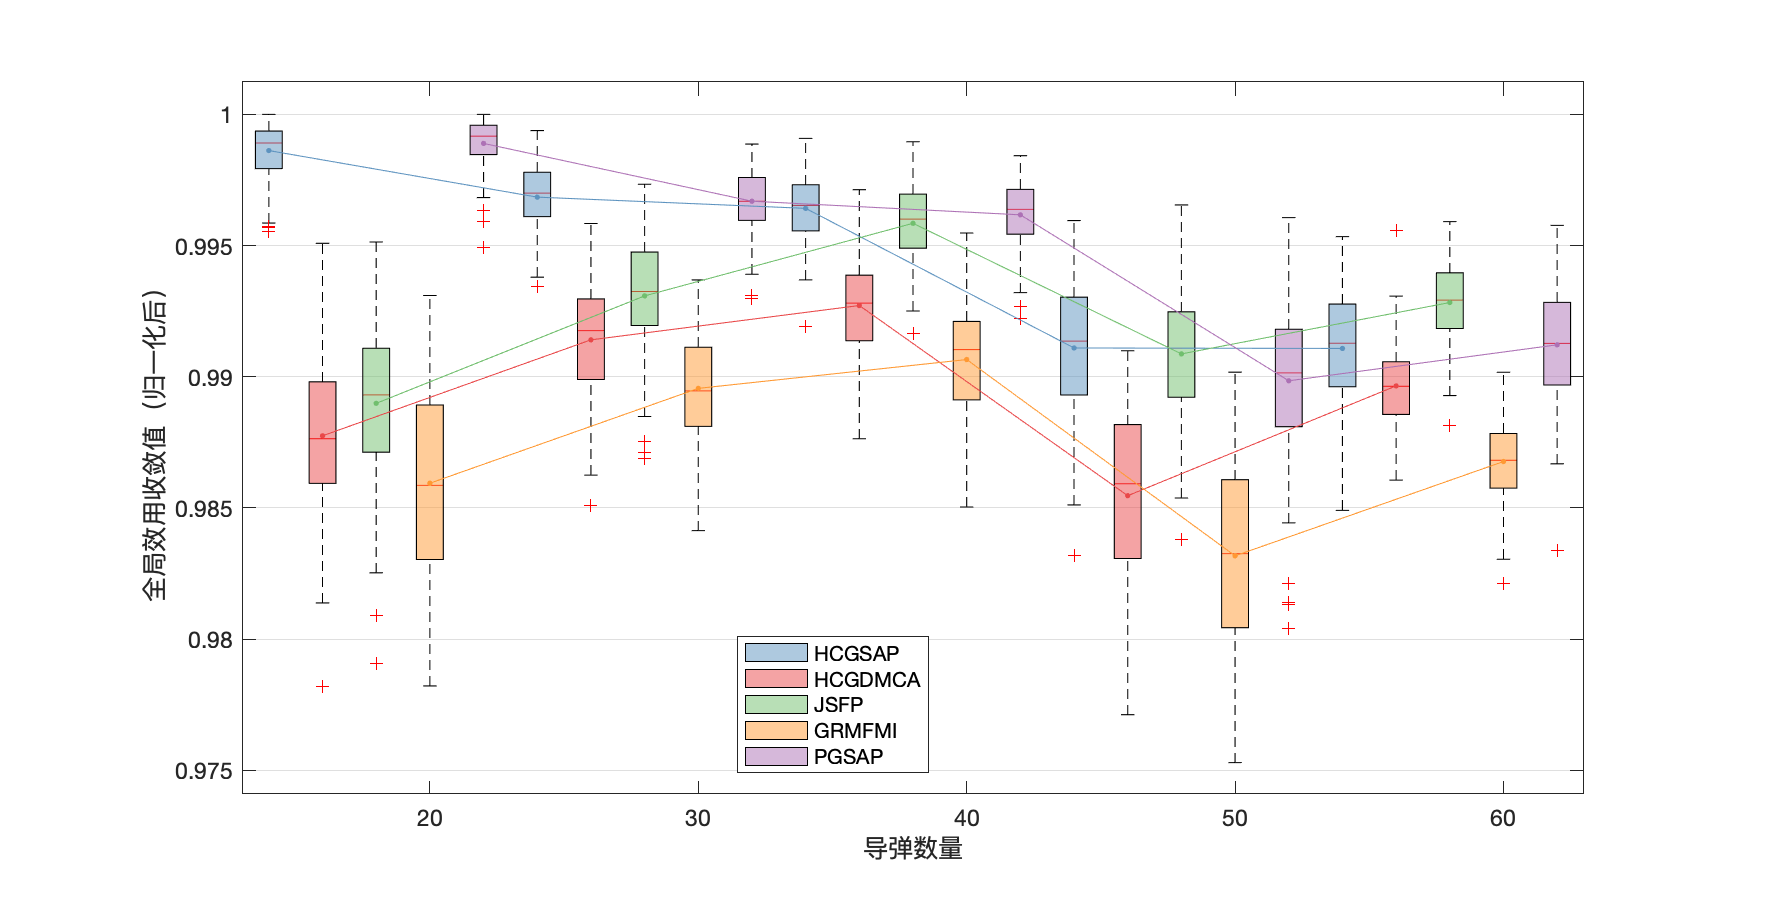
\includegraphics[height=8cm]{hedonic_game/BoxUnbalanceV1}
  \bicaption[目标数量为10的非平衡指派场景下算法优化效果对比]
    {目标数量为10的非平衡指派场景下算法优化效果对比}
    {Comparison of performance in unbalance scenarios with 10 targets}
  \label{fig:unbalance_10Targets}
\end{figure}


\begin{table}[!hpt]
  \bicaption[固定目标数量为10的非平衡指派场景下算法优化效果对比表]
  {固定目标数量为10的非平衡指派场景下算法性能对比表}
  {Comparison of algorithms' performance in unbalance scenarios with 10 targets}
  \label{tab:unbalance_10Targets}
  \centering
  %\resizebox{\textwidth}{!}{
  	\begin{tabular}{ccccccc} 
  		\toprule
    \multicolumn{2}{c}{场景} & HCGSAP & HCGDMCA & JSFP & GRMFMI & PGSAP \\
	\midrule
    \multirow{3}*{20vs10}  & 平均值 & \underline{0.9986} & 0.9877 & 0.9890 & 0.9859 & \textbf{0.9989}\\
                           & 最大值 & \underline{1}      & 0.9951 & 0.9951 & 0.9931 & \textbf{1}\\
                           & 最小值 & \textbf{0.9955} & 0.9782 & 0.9791 & 0.9782 & \underline{0.9949}\\
    \midrule
    \multirow{3}*{30vs10}  & 平均值 & \textbf{0.9968} & 0.9914 & 0.9931 & 0.9896 & \underline{0.9967}\\
    					   & 最大值 & \textbf{0.9994} & 0.9958 & 0.9973 & 0.9937 & \underline{0.9989}\\
    					   & 最小值 & \textbf{0.9935} & 0.9851 & 0.9896 & 0.9841 & \underline{0.9930}\\
    \midrule
    \multirow{3}*{40vs10}  & 平均值 & \textbf{0.9964} & 0.9927 & 0.9958 & 0.9907 & \underline{0.9962}\\
                           & 最大值 & \textbf{0.9991} & 0.9971 & \underline{0.9990} & 0.9955 & 0.9984\\
                           & 最小值 & \underline{0.9919} & 0.9876 & 0.9916 & 0.9850 & \textbf{0.9922}\\
    \midrule
    \multirow{3}*{50vs10}  & 平均值 & \textbf{0.9911} & 0.9855 & \underline{0.9909} & 0.9832 & 0.9898\\
                           & 最大值 & \underline{0.9960} & 0.9910 & 0.9937 & 0.9902 & \textbf{0.9961}\\
                           & 最小值 & \textbf{0.9832} & 0.9771 & \underline{0.9830} & 0.9753 & 0.9804\\
    \midrule
    \multirow{3}*{60vs10}  & 平均值 & 0.9911 & 0.9897 & \textbf{0.9928} & 0.9868 & \underline{0.9912}\\
                           & 最大值 & 0.9953 & 0.9956 & \textbf{0.9959} & 0.9902 & \underline{0.9958}\\
                           & 最小值 & 0.9849 & \underline{0.9861} & \textbf{0.9881} & 0.9821 & 0.9834\\
    \bottomrule
  \end{tabular}
  %}
\end{table}

\begin{figure}[!htp]
  \centering
  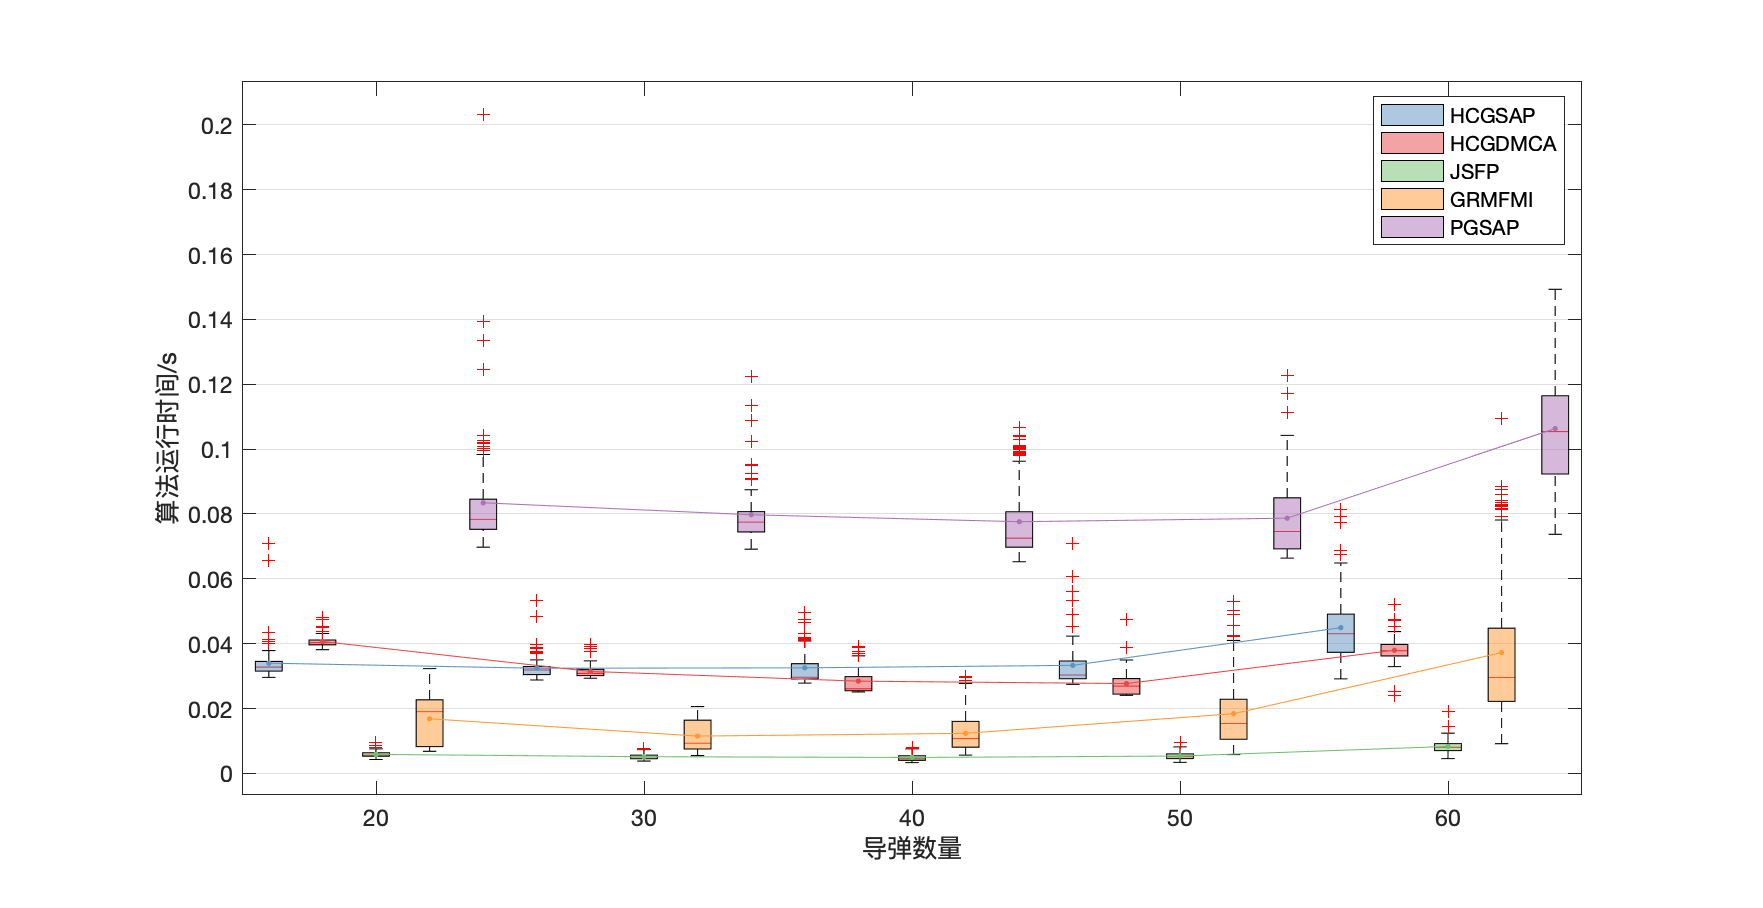
\includegraphics[height=8cm]{hedonic_game/BoxUnbalanceTimeV1}
  \bicaption[目标数量为10,不同导弹数量场景下算法运行时间对比]
    {目标数量为10,不同导弹数量场景下算法运行时间对比}
    {Comparison of running time in the scenarios with 20 targets}
  \label{fig:20TargetsTime}
\end{figure}



  
  \begin{table}[!hpt]
  \bicaption[固定目标数量为10的分配场景下算法运行时间对比表]
  {固定目标数量为10的分配场景下算法运行时间对比表(单位:s)}
  {Comparison of running time in unbalance scenarios with 10 targets (unit: s)}
  \label{tab:20Targets_time}
  \centering
  %\resizebox{\textwidth}{!}{
	\begin{tabular}{ccccccc} 
  		\toprule
    \multicolumn{2}{c}{场景} & HCGSAP & HCGDMCA & JSFP & GRMFMI & PGSAP\\
	\midrule
    \multirow{3}*{20vs10}  & 平均值 & 0.0340 & 0.0407 & 0.0058 & 0.0168 & 0.0834\\
                           & 最大值 & 0.0708 & 0.0482 & 0.0095 & 0.0323 & 0.2032\\
                           & 最小值 & 0.0296 & 0.0381 & 0.0043 & 0.0068 & 0.0698\\
    \midrule
    \multirow{3}*{30vs10}  & 平均值 & 0.0324 & 0.0314 & 0.0051 & 0.0115 & 0.0798\\
    					   & 最大值 & 0.0533 & 0.0398 & 0.0077 & 0.0206 & 0.1223\\
    					   & 最小值 & 0.0288 & 0.0293 & 0.0038 & 0.0055 & 0.0691\\
    \midrule
    \multirow{3}*{40vs10}  & 平均值 & 0.0325 & 0.0284 & 0.0049 & 0.0123 & 0.0776\\
                           & 最大值 & 0.0495 & 0.0391 & 0.0081 & 0.0297 & 0.1065\\
                           & 最小值 & 0.0278 & 0.0251 & 0.0033 & 0.0056 & 0.0653\\
    \midrule
    \multirow{3}*{50vs10}  & 平均值 & 0.0333 & 0.0277 & 0.0053 & 0.0184 & 0.0787\\
                           & 最大值 & 0.0710 & 0.0475 & 0.0096 & 0.0530 & 0.1226\\
                           & 最小值 & 0.0275 & 0.0240 & 0.0034 & 0.0058 & 0.0664\\
    \midrule
    \multirow{3}*{60vs10}  & 平均值 & 0.0449 & 0.0380 & 0.0083 & 0.0372 & 0.1063\\
                           & 最大值 & 0.0812 & 0.0521 & 0.0190 & 0.1094 & 0.1750\\
                           & 最小值 & 0.0291 & 0.0239 & 0.0045 & 0.0092 & 0.0737\\
    \bottomrule
  \end{tabular}
  %}
\end{table}






\subsection{目标之间分配数量非平衡程度影响仿真分析}
\label{hcg:sim:target_num_unbalance}

为了研究目标之间分配数量差异,即式(\ref{hcg:pro:eq:etapie})中使用的$b_{\text{max}}$对算法带来的影响,本节的仿真场景设置为在20vs10的场景下对目标取不同的$b_{\text{max}}$值。在20vs10的场景下,$b_{\text{max}}$的取值范围为$[2,11]$,即一个临界情况是当$b_{\text{max}}=2$时,意味着所有目标都被平均分配两枚导弹;另一个临界情况是当$b_{\text{max}}=11$时,意味着只有一个目标可被分配11枚导弹,其余9个目标只能被分配一枚导弹。

图\ref{fig:20vs10bmax}展示的是$b_{\text{max}}$从2变化到11的过程中,不同算法重复运行100次得到的优化结果。需要说明的是,由于在部分场景下JSFP算法最终没有收敛到可行解,因此图\ref{fig:20vs10bmax}中展示的JSFP曲线只统计了其得到可行解的优化效果。除了JSFP算法外,其余四种算法均可收敛到较好结果,其具体性能数据如表\ref{tab:20vs10bmax}所示。表中加粗数据为表现最好的算法,下划线为排名第二的算法,由此可见势博弈模型和HCG模型下的SAP算法都取得了较好的效果,而HCG模型下的DMCA算法和势博弈模型下的GRMFMI算法表现在伯仲之间。



\begin{figure}[!htp]
  \centering
  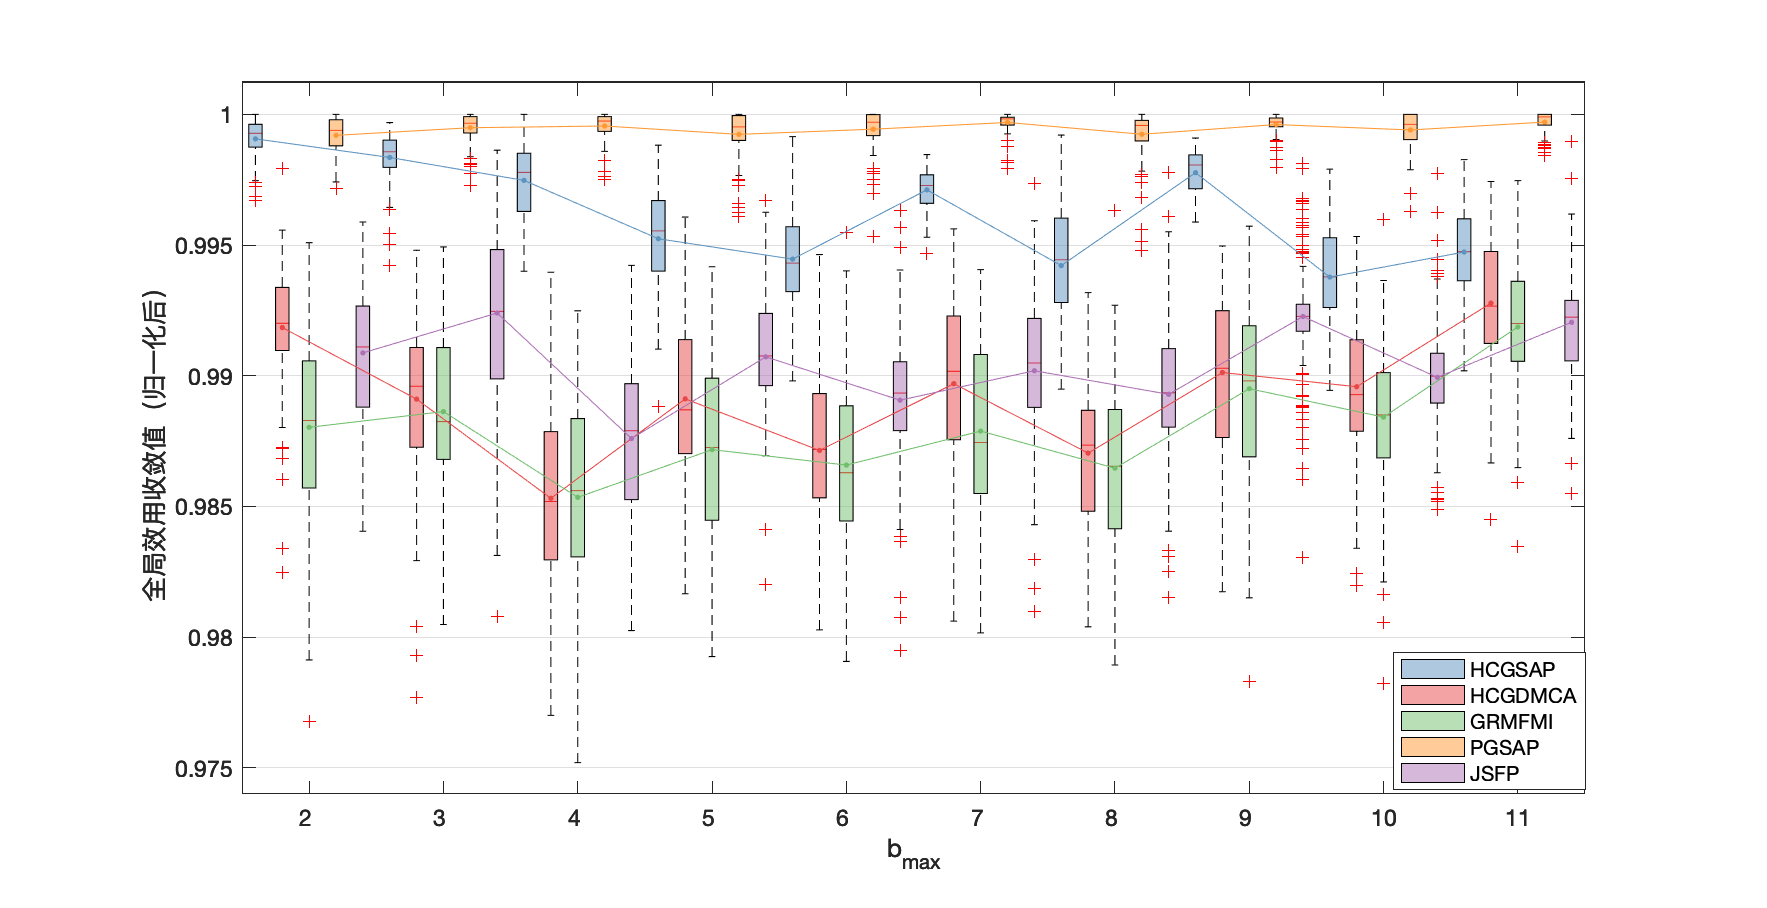
\includegraphics[height=8cm]{hedonic_game/BoxUnbalanceBmaxV2}
  \bicaption[20vs10场景的不同$b_{\text{max}}$条件下算法优化效果对比]
    {20vs10场景的不同$b_{\text{max}}$条件下算法优化效果对比}
    {Comparison of performance in 20vs10 scenarios with different $b_{\text{max}}$}
  \label{fig:20vs10bmax}
\end{figure}

\begin{figure}[!htp]
  \centering
  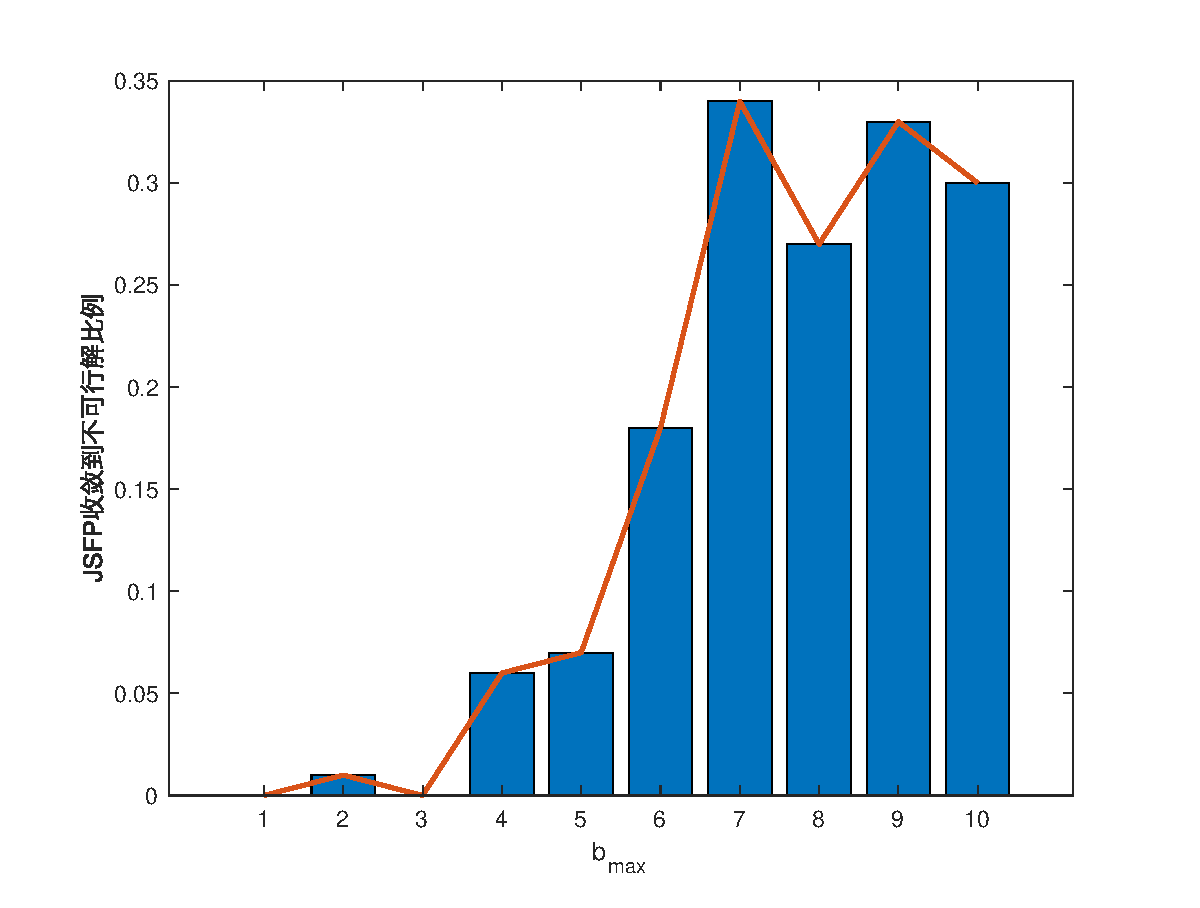
\includegraphics[height=8cm]{hedonic_game/JSFP_zeros}
  \bicaption[不同$b_{\text{max}}$条件下JSFP算法收敛到不可行解比例变化图]
    {不同$b_{\text{max}}$条件下JSFP算法收敛到不可行解比例变化图}
    {Ratio of optimizations in which JSFP converges to an in feasible solution}
  \label{fig:JSFP_zeros}
\end{figure}


从不同场景的表现稳定性来看,除了JSFP算法外,其余四种算法面对不同非平衡程度的场景表现总体稳定。图\ref{fig:JSFP_zeros}显示了JSFP算法随着$b_{\text{max}}$的增大,收敛到不可行解的次数也在增加,最高可接近35\%的迭代过程中会收敛到不可行解。总体而言,PGSAP算法的稳定性最好,其次为HCGSAP算法,HCGDMCA和GMRFMI的优化结果的分散程度相对较大,JSFP算法因为存在收敛到不可行解的情况,因此排名最后。

图\ref{fig:20vs10bmax_time}展示的是不同$b_{\text{max}}$场景下的算法运行时间对比图。从图中可直接得到的结论是HCGDMCA和GRMFMI算法运行最快,其次为HCGSAP算法,表\ref{tab:20vs10bmax_time}的数据印证了这一结论。分析PGSAP和HCGSAP运行时间较长的原因为在本文提出的任务交易机制,在导弹局部达到均衡状态后,由于任务的交易,导致算法没有收敛,因此相较于没有任务交易机制的HCGDMCA和GRMFMI算法,PGSAP和HCGSAP算法的运行时间更长。

\begin{figure}[!htp]
  \centering
  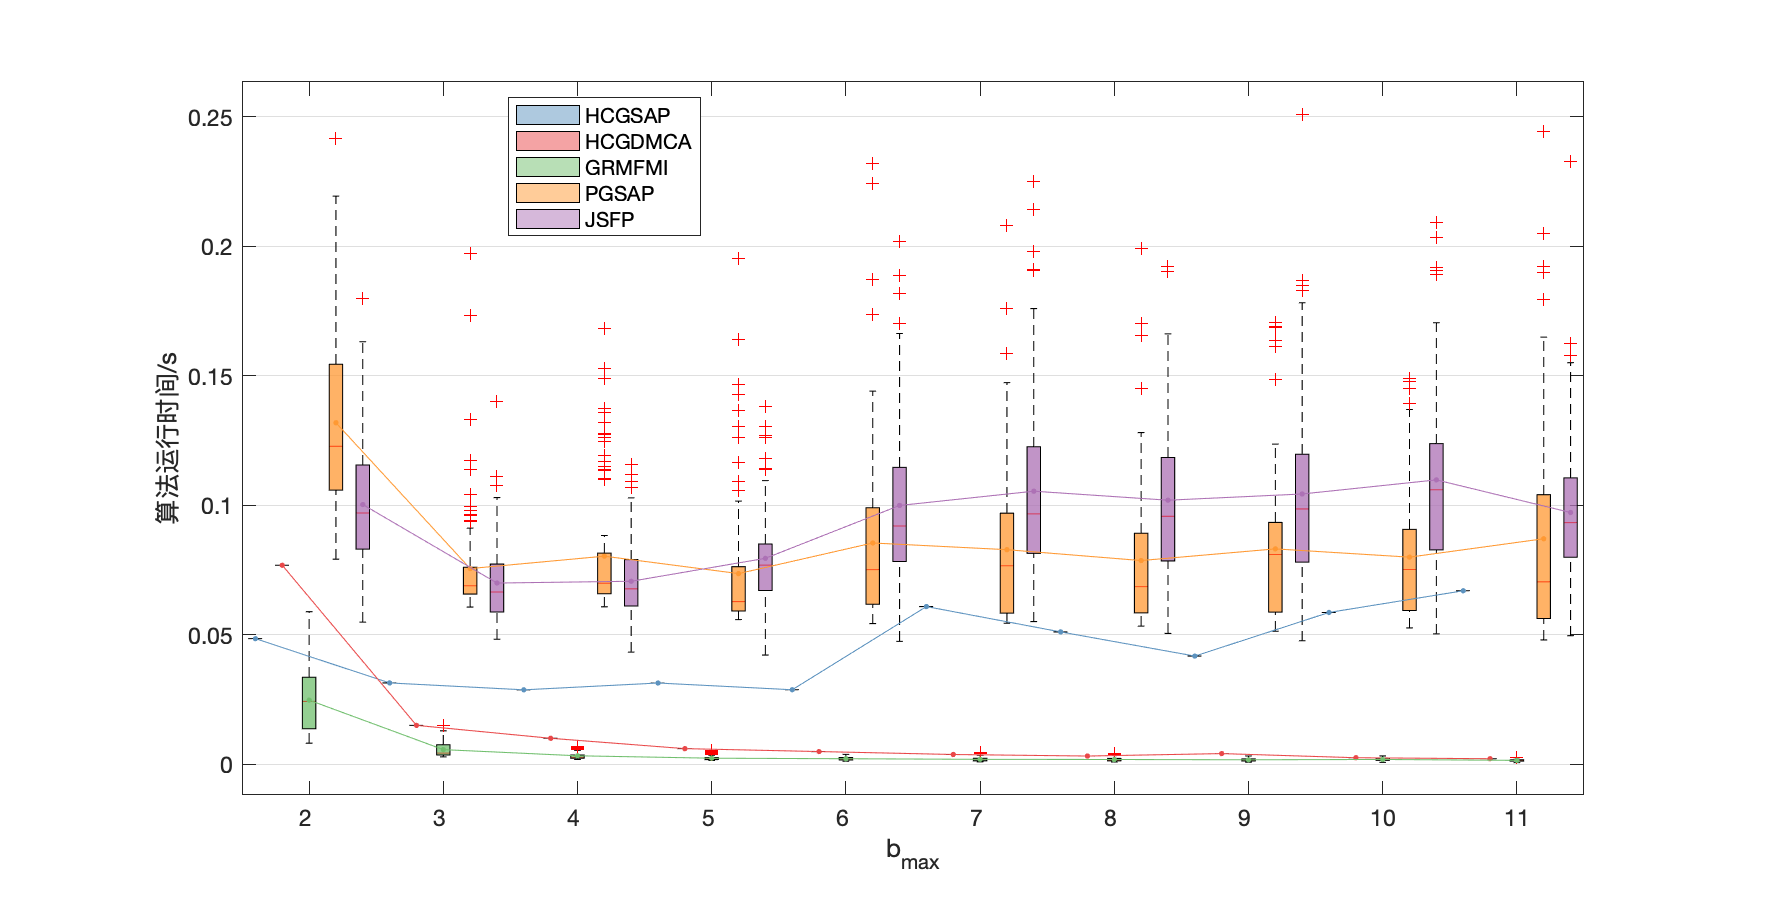
\includegraphics[height=8cm]{hedonic_game/BoxUnbalanceBmaxTimeV2}
  \bicaption[20vs10场景的不同$b_{\text{max}}$条件下算法运行时间对比]
    {20vs10场景的不同$b_{\text{max}}$条件下算法运行时间对比}
    {Comparison of running time in 20vs10 scenarios with different $b_{\text{max}}$}
  \label{fig:20vs10bmax_time}
\end{figure}


从图表可得到的第二个结论是中在$b_{\text{max}}$较小时,随着$b_{\text{max}}$的增大,几种算法的运行时间有下降的趋势,但当$b_{\text{max}}$较大时,算法运行时间基本保持不变。分析原因在于当$b_{\text{max}}$较小时,目标之间分配导弹的数量相差不大,且根据本文模型的设计,导弹在每次决策时有较多目标可以选择,因此需要迭代更多次数才能达到纳什均衡状态;而当$b_{\text{max}}$较大时,目标之间分配导弹的数量差距变大,越来越多的目标只能被一枚导弹选中,此时根据模型机制的设计\footnote{主要是由于式\ref{pg:eq:newAgentU}和式\ref{hcg:eq:agentU}的设计。},已有导弹选择的目标基本不会再被其他导弹选中,因此导弹的可选目标集变小,所有导弹会更快达到纳什均衡状态。但这样的副作用是导致算法过早收敛,陷入局部最优而无法跳出,\ref{fig:20vs10bmax}和\ref{tab:20vs10bmax}也证明了HCGDMCA和GRMFMI算法的效果相对较差。而PGSAP和HCGSAP算法由于任务交易机制的存在,使得算法可以避免这种过早收敛。

综上所述,根据两种指派问题非平衡程度的仿真实验结果可知,在面对非平衡指派问题时,本文介绍的两种博弈模型,五种算法总体上表现较好,其中本文提出的改进SAP算法可以相对来说可以得到更好的分配解,且在实时性上仍没有失去优势。HCGDMCA和GRMFMI算法虽然优化效果相比两种模型下的SAP算法较差,但仍可在大多数场景下得到97\%以上的优化效果,且实时性优势突出。JSFP算法虽然优化能力较强,但在分配问题的非平衡程度较大时,会存在收敛到不可行解的情况。



\begin{table}[!hpt]
  \bicaption[20vs10场景的不同$b_{\text{max}}$条件下算法性能对比表]
  {20vs10场景的不同$b_{\text{max}}$条件下算法性能对比表}
  {Table of comparison of performance in 20vs10 scenarios with different $b_{\text{max}}$}
  \label{tab:20vs10bmax}
  \centering
  %\resizebox{\textwidth}{!}{
  	\begin{tabular}{ccccccc} 
  		\toprule
                                       &       & HCGSAP & HCGDMCA & JSFP & GRMFMI & PGSAP\\
	\midrule
    \multirow{3}*{$b_{\text{max}}=2$}  & 平均值 & \underline{0.9991} & 0.9918 & 0.9909 & 0.9880 & \textbf{0.9992}\\
                                       & 最大值 & \underline{1}      & 0.9979 & 0.9959 & 0.9951 & \underline{1}     \\
                                       & 最小值 & \underline{0.9967} & 0.9825 & 0.9841 & 0.9768 & \textbf{0.9972}\\
    \midrule
    \multirow{3}*{$b_{\text{max}}=3$}  & 平均值 & \underline{0.9984} & 0.9891 & 0.9825 & 0.9886 & \textbf{0.9995}\\
    					               & 最大值 & \underline{0.9997} & 0.9948 & 0.9986 & 0.9949 & \textbf{1}     \\
    					               & 最小值 & \underline{0.9942} & 0.9777 & 0      & 0.9805 & \textbf{0.9973}\\
    \midrule
    \multirow{3}*{$b_{\text{max}}=4$}  & 平均值 & \underline{0.9975} & 0.9853 & 0.9876 & 0.9853 & \textbf{0.9996}\\
                                       & 最大值 & \underline{1}      & 0.9940 & 0.9942 & 0.9925 & \textbf{1}     \\
                                       & 最小值 & \underline{0.9940} & 0.9770 & 0.9803 & 0.9752 & \textbf{0.9975}\\
    \midrule
    \multirow{3}*{$b_{\text{max}}=5$}  & 平均值 & \underline{0.9952} & 0.9891 & 0.8916 & 0.9872 & \textbf{0.9992}\\
                                       & 最大值 & \underline{0.9988} & 0.9961 & 0.9967 & 0.9942 & \textbf{1}     \\
                                       & 最小值 & \underline{0.9888} & 0.9817 & 0      & 0.9793 & \textbf{0.9961}\\
    \midrule
    \multirow{3}*{$b_{\text{max}}=6$}  & 平均值 & \underline{0.9945} & 0.9871 & 0.8802 & 0.9866 & \textbf{0.9994}\\
                                       & 最大值 & \underline{0.9992} & 0.9946 & 0.9963 & 0.9955 & \textbf{1}     \\
                                       & 最小值 & \underline{0.9898} & 0.9803 & 0      & 0.9791 & \textbf{0.9953}\\
    \midrule
    \multirow{3}*{$b_{\text{max}}=7$}  & 平均值 & \underline{0.9971} & 0.9897 & 0.8614 & 0.9879 & \textbf{0.9997}\\
                                       & 最大值 & \underline{0.9985} & 0.9956 & 0.9973 & 0.9941 & \textbf{1}     \\
                                       & 最小值 & \underline{0.9947} & 0.9806 & 0      & 0.9802 & \textbf{0.9979}\\
    \midrule
    \multirow{3}*{$b_{\text{max}}=8$}  & 平均值 & \underline{0.9942} & 0.9870 & 0.7222 & 0.9865 & \textbf{0.9992}\\
                                       & 最大值 & \underline{0.9992} & 0.9932 & 0.9978 & 0.9963 & \textbf{1}     \\
                                       & 最小值 & \underline{0.9895} & 0.9804 & 0      & 0.9789 & \textbf{0.9948}\\
    \midrule
    \multirow{3}*{$b_{\text{max}}=9$}  & 平均值 & \underline{0.9978} & 0.9901 & 0.6251 & 0.9895 & \textbf{0.9996}\\
                                       & 最大值 & \underline{0.9991} & 0.9950 & 0.9981 & 0.9957 & \textbf{1}     \\
                                       & 最小值 & \underline{0.9959} & 0.9817 & 0      & 0.9783 & \textbf{0.9980}\\
    \midrule
    \multirow{3}*{$b_{\text{max}}=10$}  & 平均值 & \underline{0.9938} & 0.9896 & 0.7028 & 0.9884 & \textbf{0.9994}\\
                                        & 最大值 & \underline{0.9979} & 0.9953 & 0.9978 & 0.9960 & \textbf{1}     \\
                                        & 最小值 & \underline{0.9894} & 0.9820 & 0      & 0.9782 & \textbf{0.9963}\\
    \midrule
    \multirow{3}*{$b_{\text{max}}=11$}  & 平均值 & \underline{0.9938} & 0.9928 & 0.6051 & 0.9919 & \textbf{0.9997}\\
                                        & 最大值 & \underline{0.9979} & 0.9974 & 0.9990 & 0.9975 & \textbf{1}\\
                                        & 最小值 & \underline{0.9894} & 0.9845 & 0      & 0.9835 & \textbf{0.9984}\\
    \bottomrule
  \end{tabular}
  %}
\end{table}



  
  \begin{table}[!hpt]
  \bicaption[20vs10场景的不同$b_{\text{max}}$条件下算法运行时间对比表]
  {20vs10场景的不同$b_{\text{max}}$条件下算法运行时间对比表(单位:s)}
  {Table of comparison of running time in 20vs10 scenarios with different $b_{\text{max}}$ (unit: s)}
  \label{tab:20vs10bmax_time}
  \centering
  %\resizebox{\textwidth}{!}{
	\begin{tabular}{ccccccc} 
  		\toprule
                                       &       & HCGSAP & HCGDMCA & JSFP & GRMFMI & PGSAP\\
	\midrule
    \multirow{3}*{$b_{\text{max}}=2$}  & 平均值 & 0.0484 & 0.0205 & 0.1002 & 0.0247 & 0.1318\\
                                       & 最大值 & 0.0612 & 0.0268 & 0.1796 & 0.0588 & 0.2416\\
                                       & 最小值 & 0.0304 & 0.0179 & 0.0548 & 0.0081 & 0.0791\\
    \midrule
    \multirow{3}*{$b_{\text{max}}=3$}  & 平均值 & 0.0328 & 0.0182 & 0.0678 & 0.0058 & 0.0852\\
    					               & 最大值 & 0.0600 & 0.0257 & 0.1336 & 0.0162 & 0.2017\\
    					               & 最小值 & 0.0267 & 0.0161 & 0.0439 & 0.0026 & 0.0646\\
    \midrule
    \multirow{3}*{$b_{\text{max}}=4$}  & 平均值 & 0.0331 & 0.0094 & 0.0750 & 0.0033 & 0.0753\\
                                       & 最大值 & 0.0675 & 0.0141 & 0.1292 & 0.0082 & 0.2237\\
                                       & 最小值 & 0.0231 & 0.0084 & 0.0517 & 0.0016 & 0.0581\\
    \midrule
    \multirow{3}*{$b_{\text{max}}=5$}  & 平均值 & 0.0284 & 0.0073 & 0.0842 & 0.0024 & 0.0801\\
                                       & 最大值 & 0.0535 & 0.0106 & 0.1473 & 0.0065 & 0.1733\\
                                       & 最小值 & 0.0246 & 0.0068 & 0.0536 & 0.0013 & 0.0600\\
    \midrule
    \multirow{3}*{$b_{\text{max}}=6$}  & 平均值 & 0.0275 & 0.0053 & 0.0852 & 0.0017 & 0.0797\\
                                       & 最大值 & 0.0438 & 0.0081 & 0.1633 & 0.0043 & 0.1894\\
                                       & 最小值 & 0.0231 & 0.0051 & 0.0511 & 0.0010 & 0.0560\\
    \midrule
    \multirow{3}*{$b_{\text{max}}=7$}  & 平均值 & 0.0301 & 0.0040 & 0.0873 & 0.0017 & 0.0754\\
                                       & 最大值 & 0.0465 & 0.0042 & 0.1577 & 0.0037 & 0.1751\\
                                       & 最小值 & 0.0226 & 0.0039 & 0.0504 & $<10^{-3}$ & 0.0545\\
    \midrule
    \multirow{3}*{$b_{\text{max}}=8$}  & 平均值 & 0.0356 & 0.0035 & 0.0912 & 0.0016 & 0.0777\\
                                       & 最大值 & 0.0808 & 0.0050 & 0.1815 & 0.0030 & 0.1849\\
                                       & 最小值 & 0.0225 & 0.0034 & 0.0507 & $<10^{-3}$ & 0.0548\\
    \midrule
    \multirow{3}*{$b_{\text{max}}=9$}  & 平均值 & 0.0444 & 0.0028 & 0.0894 & 0.0016 & 0.0811\\
                                       & 最大值 & 0.0801 & 0.0040 & 0.1401 & 0.0039 & 0.1607\\
                                       & 最小值 & 0.0220 & 0.0027 & 0.0524 & $<10^{-3}$ & 0.0527\\
    \midrule
    \multirow{3}*{$b_{\text{max}}=10$}  & 平均值 & 0.0465 & 0.0028 & 0.1034 & 0.0016 & 0.0887\\
                                        & 最大值 & 0.0877 & 0.0040 & 0.2011 & 0.0030 & 0.2559\\
                                        & 最小值 & 0.0210 & 0.0027 & 0.0489 & $<10^{-3}$ & 0.0531\\
    \midrule
    \multirow{3}*{$b_{\text{max}}=11$}  & 平均值 & 0.0576 & 0.0023 & 0.0977 & 0.0016 & 0.0950\\
                                        & 最大值 & 0.0887 & 0.0034 & 0.1938 & 0.0030 & 0.2268\\
                                        & 最小值 & 0.0327 & 0.0020 & 0.0261 & $<10^{-3}$ & 0.0509\\
    \bottomrule
  \end{tabular}

  %}
\end{table}

\section{本章小结}
\label{hg:sec:conclusion}

本章将任务分配问题看作联盟形成过程,建立了基于偏好联盟博弈模型(HCG)的任务分配算法,并介绍了两种基于该模型的学习算法:改进SAP算法和针对HCG模型的分布式一致性算法(DMCA)。在设计智能体效用函数时,假设智能体满足社交疏远性质,并针对约束条件改进智能体效用函数,得到了基于HCG的分布式任务分配模型。从理论上证明了该模型的有效性、算法复杂度和最优性。使用第\ref{chap:pg}中提出的改进SAP算法和DMCA算法对HCG任务分配模型进行学习优化。通过与第\ref{chap:pg}章的势博弈学习算法共同进行仿真实验,从两种非平衡程度设计仿真试验,验证了本文使用的基于两种博弈论模型的分布式任务分配算法在非平衡问题中的有效性和突出的时间优势。




